\newpage

\section{Commande événementielle}
\label{cmd_ev}
Cette section est une rapide étude bibliographique sur la commande événementielle, dont l'implémentation est l'un des objectifs finaux du projet eSWARM. La commande évenementielle est un sujet de recherche concentrant de plus en plus d'intérêts, avec autant de papiers publiés entre 2018 et 2020 qu'entre 1999 et 2018 \cite{aranda-escolastico_event-based_2020}.

\subsection{Définition de la commande événementielle}

La commande événementielle, appelée en anglais \textit{Event-based control} ou encore \textit{Event-based paradigm}, est définie dans \cite{astrom_event_2008} comme étant une alternative au contrôle par échantillonnage périodique classique. Contrairement à ce dernier, où les actions de contrôle sont exécutées à intervalles réguliers, cette approche les déclenche uniquement lorsque certaines conditions sont remplies. Elle permet ainsi une gestion plus efficace des ressources en réduisant les opérations inutiles. Une définition similaire est donnée dans \cite{durand_event-based_2015}, ou encore dans \cite{heemels_introduction_2012}.

\noindent Il existe deux principaux types de commande événementielle \cite{aranda-escolastico_event-based_2020} : 
\begin{itemize}
    \item \textit{commande événementielle continue ou son équivalent discret} : une condition de déclenchement est surveillée en continu (ou à des instants discrets). 
    \item \textit{commande auto-déclenchée} : Une approche prédictive où, au lieu de surveiller en permanence une condition de déclenchement, l'instant du prochain événement est prédit à partir des informations actuelles et d'un modèle du système.
\end{itemize}

L'un des articles les plus importants de la commande événementiel discrète est celui de  Karl-Erik Årzén, qui introduit un premier contrôleur PID événementiel en 1999 \cite{aarzen_simple_1999}. La logique de détection des événements est basée ici sur la différence d'erreur ou le temps écoulé depuis le dernier échantillon. La condition suivante est utilisée dans son document est :
\[
  e(t_k) - e(t_s) > e_{\text{lim}} \quad \text{ou} \quad h_{\text{act}} \geq h_{\text{max}}
\]
où \( e(t_k) \) est l'erreur actuelle, \( e(t_s) \) est l'erreur précédente, et \( h_{\text{act}} \) est l'intervalle de temps écoulé depuis le dernier échantillon. Le contrôleur effectue une action de contrôle si l'une de ces deux conditions est remplie. 

Plusieurs versions améliorées de ce même contrôleur sont proposées en 2009 \cite{durand_further_2009}, l'une supprimant par exemple la condition $h_{\text{act}} \geq h_{\text{max}}$, simplifiant ainsi le système.

Pour ce qui est de la commande auto-déclenchée, elle est décrite dans \cite{aranda-escolastico_event-based_2020}  . Par exemple, \cite{trimpe_event-based_2015} propose, dans un cas simple où un ordinateur/opérateur communique avec un robot, d'implémenter des modèles de prédiction, tels qu'un filtre de Kalman étendu \cite{gangloff_mooc_2023, li_kalman_2015}, afin de réduire davantage les échanges d'informations. Dans ce cadre, le robot et l'opérateur utilisent ces prédictions pour déterminer la distribution de probabilité de l'état du robot, qui transmet ensuite ses mises à jour uniquement lorsque la prédiction de l'opérateur devient trop imprécise. 

Pour ce qui est de la commande auto-déclenchée, elle est décrite dans \cite{aranda-escolastico_event-based_2020}. Par exemple, \cite{trimpe_event-based_2015} propose, dans un cas simple où un ordinateur distant communique avec un robot, d'utiliser des modèles de prédiction pour réduire les échanges d'information. Dans ce cadre, un filtre de Kalman étendu (EKF) \cite{gangloff_mooc_2023, li_kalman_2015} est mis en œuvre à la fois pour estimer l’état courant et prédire l’état futur du robot à partir de son modèle dynamique. Cette prédiction permet à l'opérateur, qui ne reçoit pas systématiquement les nouvelles estimations du robot, de s'appuyer alors sur une estimation locale qu’il met à jour uniquement lorsque la divergence avec l’estimation réelle dépasse un certain seuil. 



\newpage

\subsection{Exemples d'application}

Une application de la commande événementielle pour piloter un quadcoptère a été réalisée \cite{durand_event-based_nodate} à l'aide d'un système de motion capture. L'objectif a été de donner plusieurs points-destinations au drone, et de l'asservir en position avec un contrôleur événementiel. Une comparaison est ensuite réalisée avec un asservissement classique, démontrant ainsi l'intérêt de la commande événementielle, puisque le nombre d'échantillons nécessaire pour asservir le drone diminue sans perte de performance avec le nouveau type de commande (à condition de ne pas mettre un seuil de déclenchement $e_{lim}$ trop grand).

Un autre article mettant en œuvre une commande événementielle dans un projet lié à la robotique est \cite{postoyan_event-triggered_2015}. Ici, les résultats montrent que cette approche permet une réduction significative des communication par rapport aux méthodes traditionnelles à déclenchement périodique. 

\cite{ding_overview_2018} propose une synthèse des avancées concernant les stratégies de contrôle évènementiel dans les systèmes multiagents. Parmi les exemples donnés dans l'article, on retrouve un microgrid (petit réseau électrique), dans lequel une commande événementielle permet de réguler la tension de chaque générateur en minimisant le nombre de communications. Les simulations montrent que le nombre total de transmissions peut être réduit de plus de 60\% par rapport à une commande périodique classique. .

Dans un autre exemple, plus proche du projet eSWARM, un essaim de robots non-holonomes a maintenu une formation géométrique cible à l’aide d’une commande événementiel dynamique, où les communications inter-robots ne sont déclenchées que lorsque certaines erreurs dépassent un seuil variable. Cette méthode a également pu réduire de manière significative de la fréquence de mise à jour des commandes, tout en maintenant la formation avec une erreur de suivi comparable à celle obtenue avec des mises à jour régulières. 

Ce document met également en avant les difficultés de l'implémentation de la commande événementielles. Cela sera développé dans la section \ref{problemes_cmd_event}.

\subsection{Intégration}

En vue d'une implémentation de la commande événementielle dans la commande d'un essaim de robot, il convient de noter que les méthodes basées sur le consensus (\cite{koung_consensus-based_2020}), sur la logique leader-follower (\cite{yang_adaptive_2021})  décrites précédemment, peuvent utiliser un PID pour asservir les différents modules de l'essaim. 
Dans cette optique, le schéma bloc classique d'un PID événementielle, tel que défini par Karl-Erik Årzén \cite{aarzen_simple_1999} est donnée Fig [\ref{fig:schema_event_based}] :
\begin{figure}[H]  % H force l'affichage à cet endroit précis
    \centering
    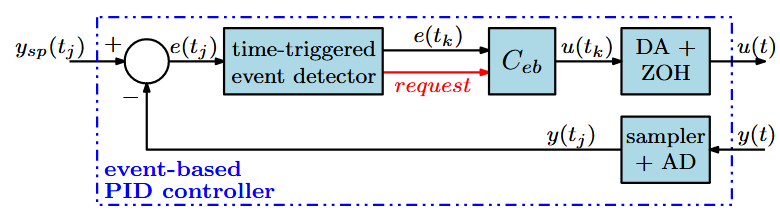
\includegraphics[scale=0.6]{8-Etat_de_art/cmd_ev/pic/event-based-control.PNG}
    \caption{Schéma d'un asservissement événementiel, sur la base de \cite{durand_event-based_nodate}}
    \label{fig:schema_event_based}  % Label pour faire référence à la figure
    \vspace{-0.3cm}
\end{figure}

\begin{itemize}
    \item Sampler + AD: Convertisseur analogique-numérique (AD) qui échantillonne le signal de sortie \( y(t) \) à des instants discrets \( t_j \) pour produire le signal échantillonné \( y(t_j) \).

    \item Event Detector: Détecteur d'événements qui compare la consigne \( y_{sp}(t_j) \) avec le signal échantillonné \( y(t_j) \) pour générer l'erreur $ e(t_j) = y_{sp}(t_j) - y(t_j)$, pour ensuite comparer cette erreur avec le seuil de détection.

    \item $C_{eb}$: Représente le contrôleur basé sur des événements. Ce contrôleur fonctionne de manière asynchrone et génère des commandes uniquement lorsque certains critères sont remplis (entrée request), et fournit une commande $u(t_k)$ 
    \item DA + ZOH: Convertisseur numérique-analogique (DA) avec maintien d'ordre zéro (ZOH) qui convertit le signal de commande discret \( u(t_j) \) en un signal continu \( u(t) \) maintenu constant pendant la période d'échantillonnage \( \bar{h} \).
\end{itemize}

\subsection{Problèmes liés à la commande événementielle}
\label{problemes_cmd_event}

Malgré ses nombreux avantages en matière de réduction des communications et d’efficacité énergétique, la commande événementielle est confrontée à certains défis qu’il convient de considérer avant toute implémentation concrète.

\subsubsection{Comportement Zeno}  
L’un des problèmes théoriques les plus critiques est le phénomène de type Zeno \cite{yu_zeno_2021}, qui se manifeste lorsqu’un nombre infini d’événements est déclenché dans un intervalle de temps fini. Cela rend la solution mathématique du système invalide au-delà d’un certain instant et empêche toute exécution physique réaliste du contrôle.

Dans le cas de systèmes multi-agents, ce comportement peut survenir notamment lorsque les déclenchements dépendent uniquement de l’état local ou de l’erreur vis-à-vis d’un modèle. Il est démontré que si le seuil d’activation des événements est défini uniquement en fonction de ces états, alors le comportement Zeno devient inévitable. En revanche, certaines approches à base de modèles prédictifs, où le seuil dépend de l’estimation de l’état global ou d’un modèle, permettent d’atténuer ce phénomène. 

Pour y remédier, plusieurs stratégies sont proposées :
\begin{itemize}
    \item imposer une borne inférieure stricte sur le temps entre deux événements ;
    \item utiliser des fonctions seuils indépendantes de l’état courant ;
\end{itemize}

\subsubsection{Explosion de la partie intégrale.}  

Une autre difficulté de la commande événementielle est "l’explosion" de la partie intégrale pendant les périodes prolongées sans événement. En effet, lorsque le système reste stable, l'intervalle de temps entre deux événements (noté $h_{\text{act}}$) peut devenir très grand. Cela entraîne une accumulation excessive de l’erreur dans la partie intégrale du contrôleur, qui, lors d’un changement soudain de consigne, provoque des dépassements importants et détériore la performance du système. Pour pallier ce problème, plusieurs solutions ont été proposées \cite{durand_further_2009}. La première consiste à saturer le produit $h \cdot e$, afin de limiter l’impact des longues périodes stables sur l’intégration. La seconde utilise un facteur d’oubli exponentiel, qui atténue progressivement l’influence des anciennes erreurs. 

 
